% slide 29: visualize results in bar chart. Select important algos and have 4 bars (each of eval. methods)
% slide xx: some more slides with e.g. zeros..
% slide xx: examples of ranking

\begin{frame}
  \frametitle{Results for NDCG@10}
  \begin{figure}[tbph]
    \centering
    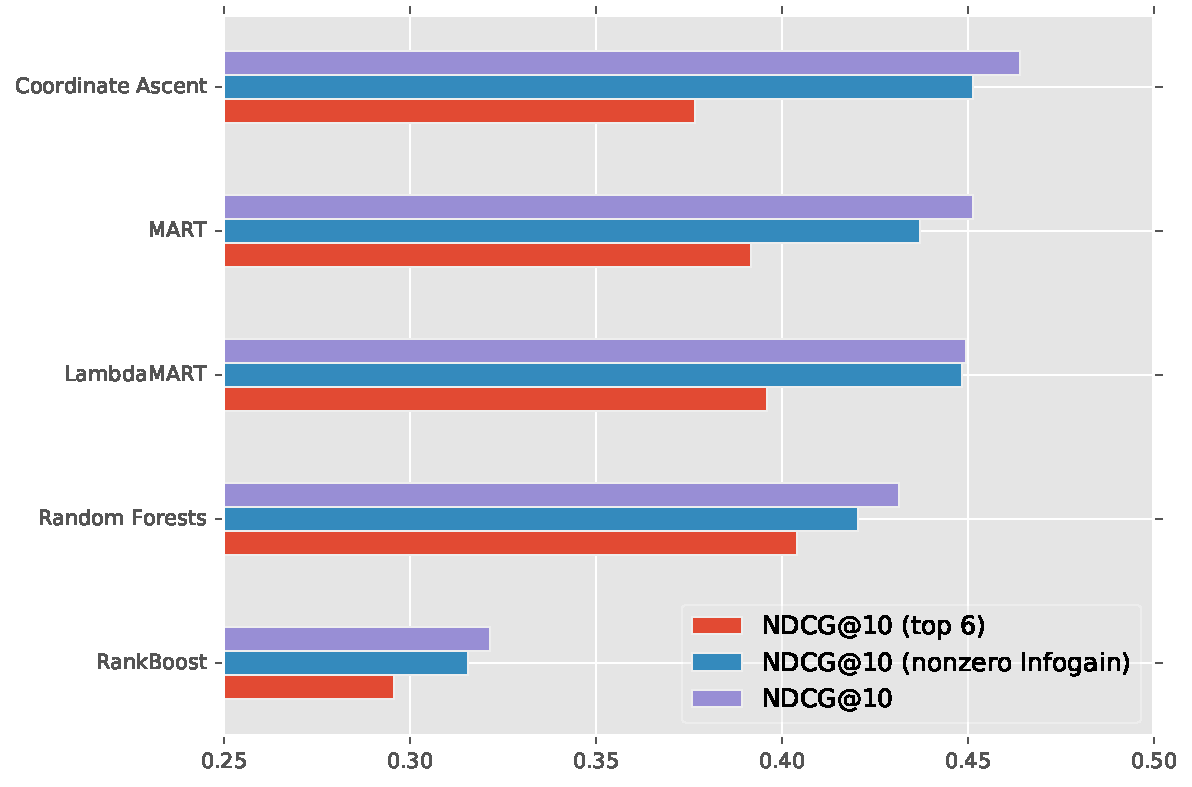
\includegraphics[width=\linewidth]{images/results_ndcg10}
  \end{figure}
\end{frame}

\begin{frame}
  \frametitle{Results for P@191}
  \begin{figure}[tbph]
    \centering
    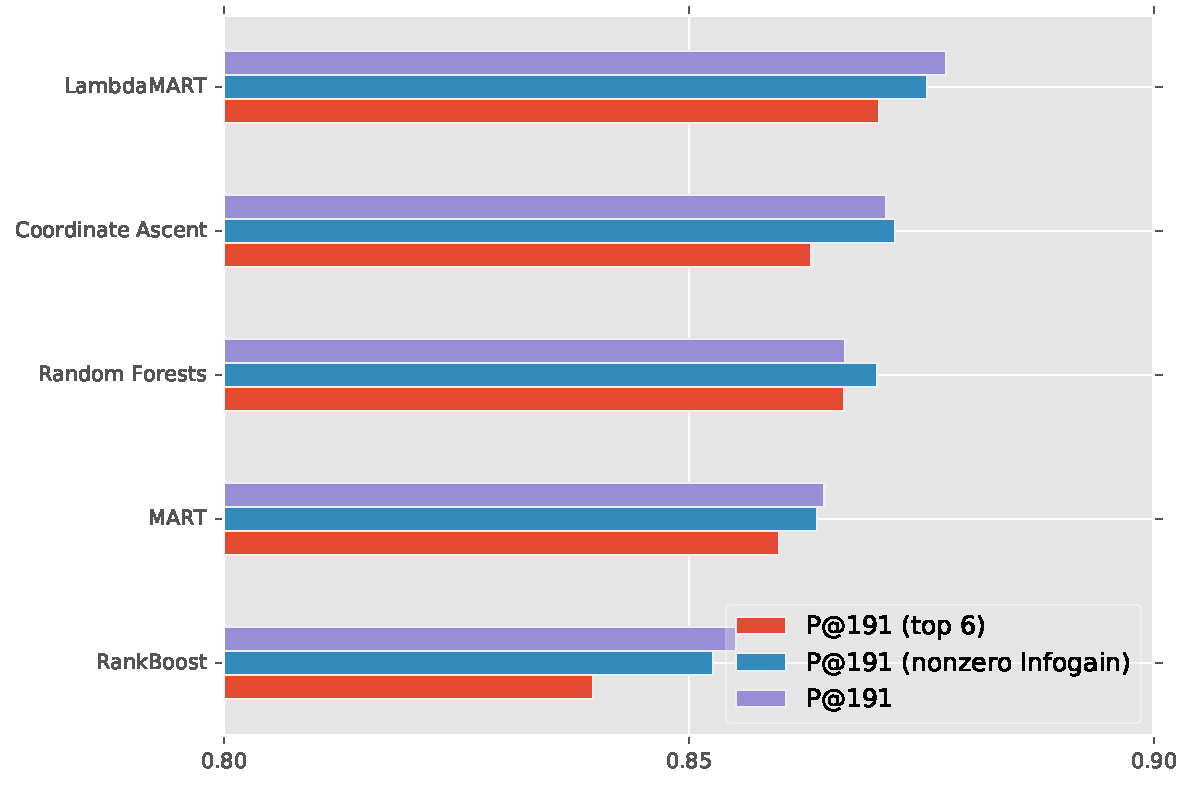
\includegraphics[width=\linewidth]{images/results_p191}
  \end{figure}
\end{frame}

\begin{frame}
  \frametitle{Results for PP@75}
  \begin{figure}[tbph]
    \centering
    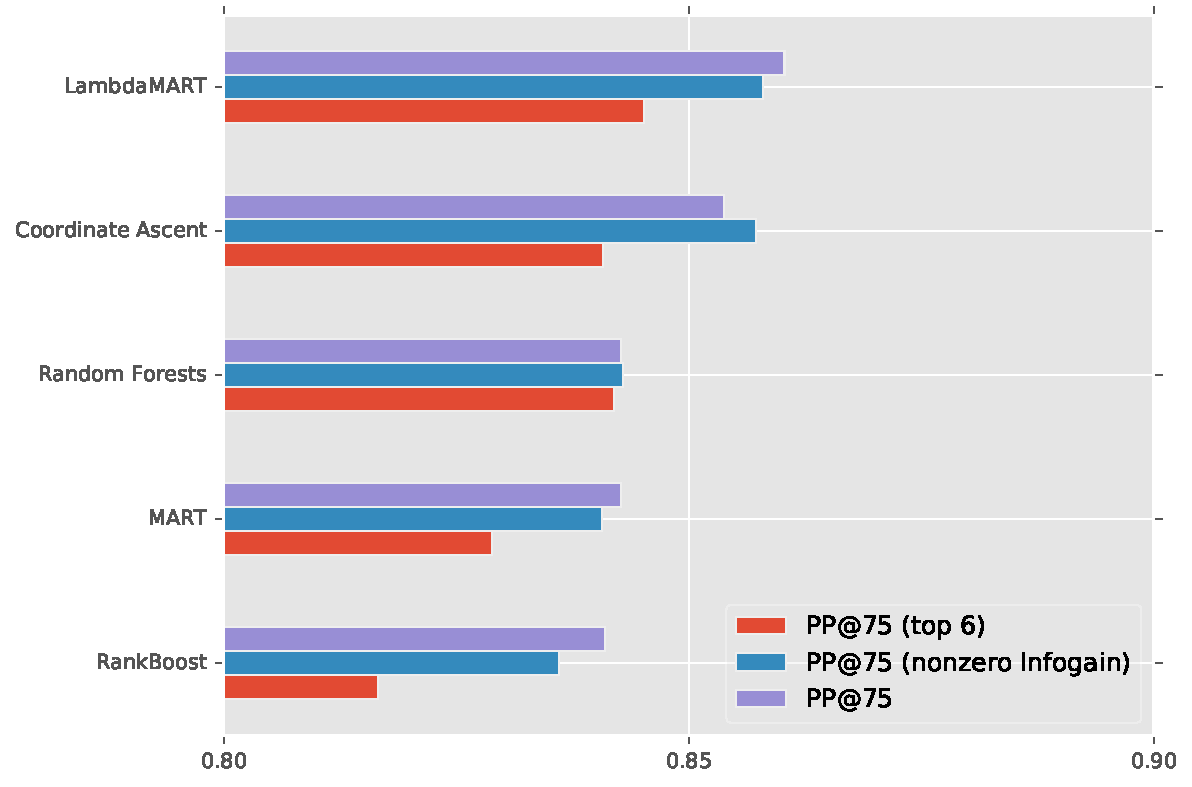
\includegraphics[width=\linewidth]{images/results_pp75}
  \end{figure}
\end{frame}

\begin{frame}
  \frametitle{Results for PP@50}
  \begin{figure}[tbph]
    \centering
    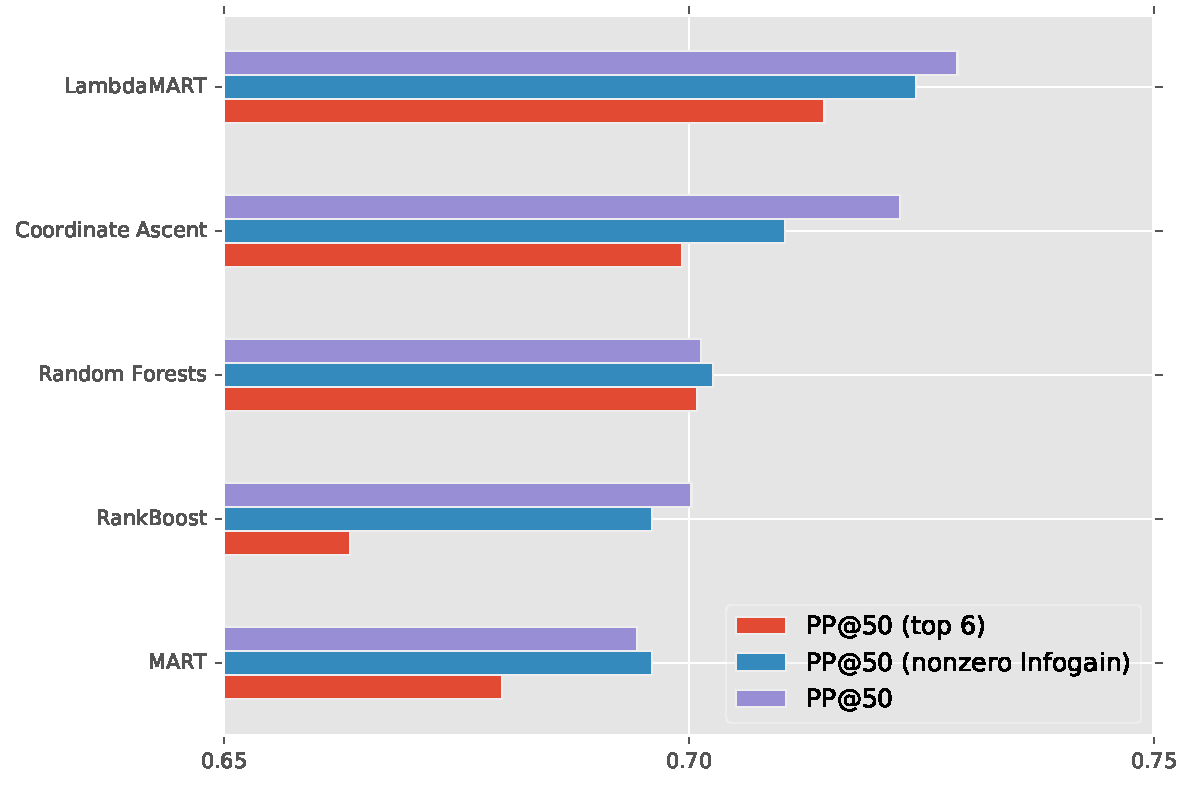
\includegraphics[width=\linewidth]{images/results_pp50}
  \end{figure}
\end{frame}

\begin{frame}
  \frametitle{Results for PP@k for various k}
  \begin{figure}[tbph]
    \centering
    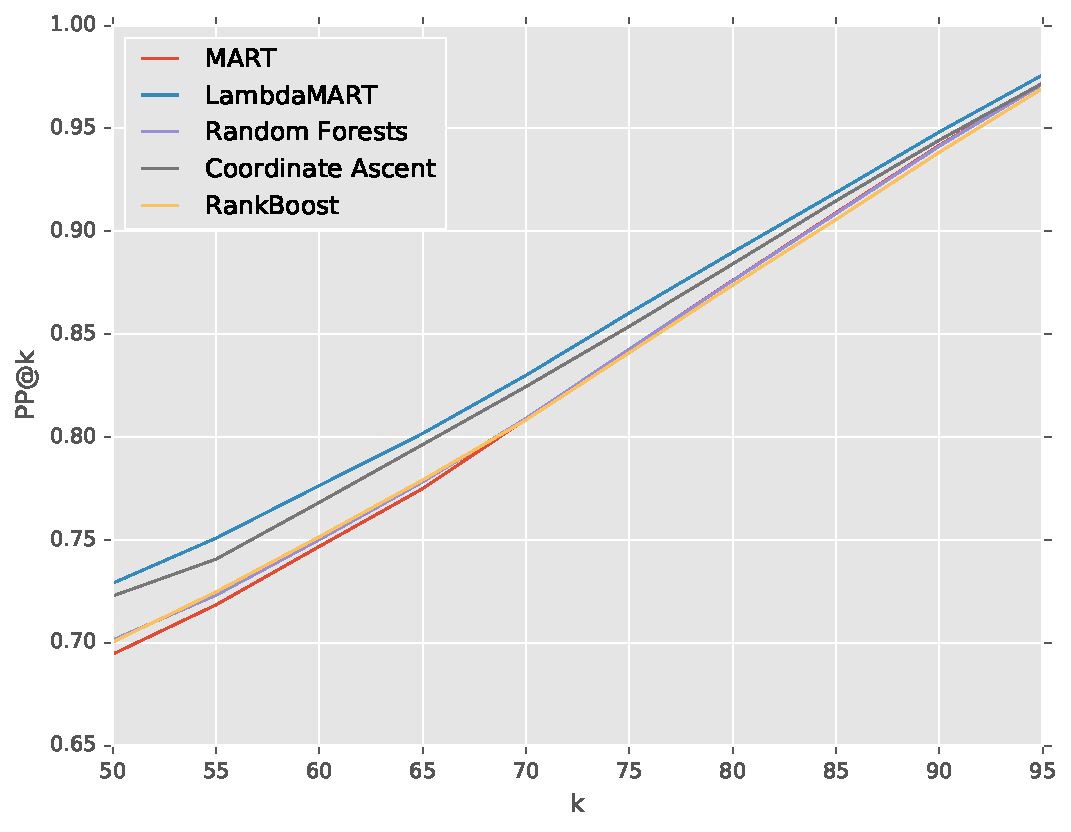
\includegraphics[width=0.95\linewidth]{images/results_pp_k}
  \end{figure}
\end{frame}

\begin{frame}
  \frametitle{Comparison of learning times}
  \begin{figure}[tbph]
    \centering
    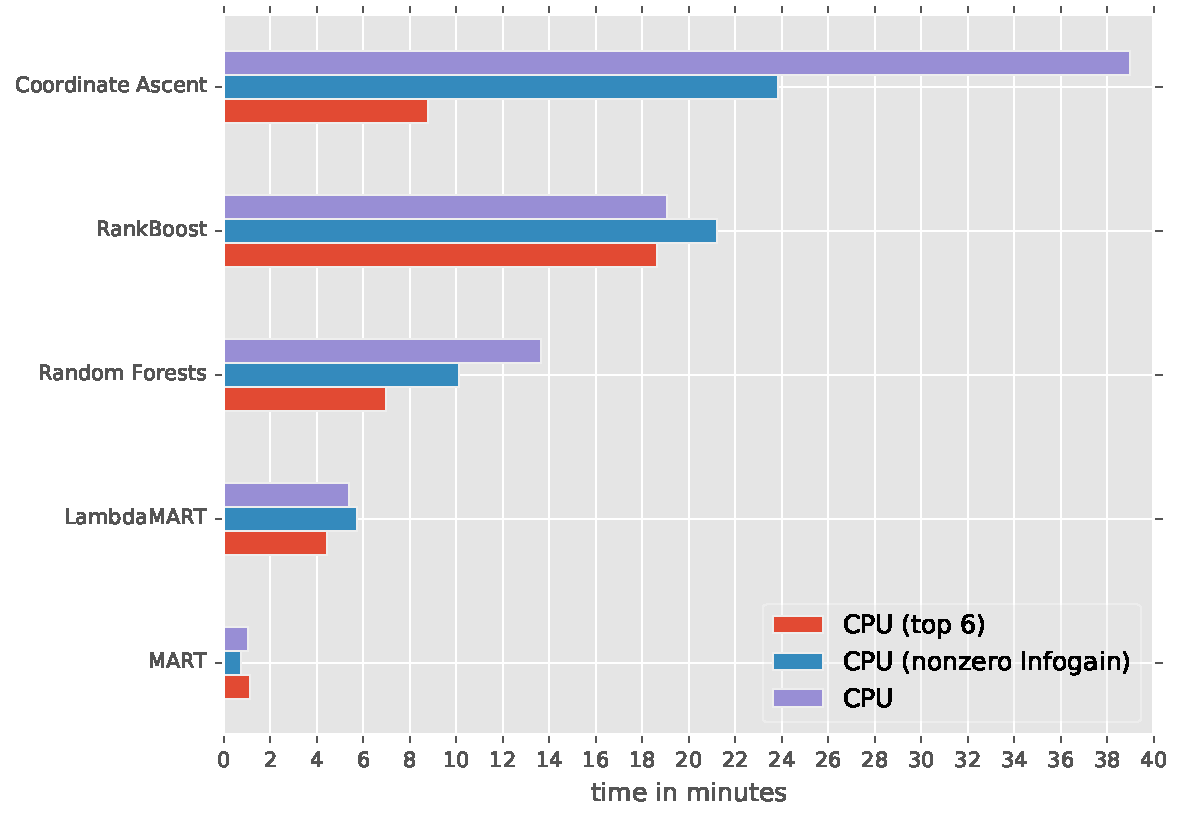
\includegraphics[width=0.95\linewidth]{images/results_times}
  \end{figure}
\end{frame}